\chapter{Autoimmune Enzephalitis und CASPR2}
\textbf{Helene Becker}
\section{Definition und Krankheitsbild}
Als Enzephalitis wird eine Entzündung des Gehirns bezeichnet.
Je nach Ursache und Ausprägung der Symptome werden verschiedene Arten
von Enzephalitiden unterschieden.

Enzephalitiden werden meist ausgelöst, indem ein Virus das Hirn direkt
infiziert oder ein Virus, ein Impfstoff oder etwas anderes die Entzündung
auslöst. Als Folge einer Viruserkrankung kann so beispielsweise eine
epidemische oder eine sporadische Enzephalitis entstehen. Ebenfalls kann
(aus einer Virusinfektion oder aus der Reaktion von T-Zellen auf einen Tumor) eine 
autoimmune Enzephalitis (AE) hervorgehen.\footcite{Klein2026}
Bei der AE handelt es sich um eine Autoimmunerkrankung, bei der es zur
fehlgeleiteten Immunabwehr gegen körpereigene neuronale Strukturen
kommt.\footcites{Klein2026}{Fernandez2026}
Dabei werden AK gegen Antigene körpereigener Gewebe durch das
Immunsystem hergestellt, jene werden dann als sogenannte aAK
bezeichnet. Eine solche Autoimmunreaktion kann zu neuronalen 
Entzündungen und Gewebeschäden führen.\footcite{Fernandez2026}

Der Begriff AE beschreibt eine Gruppe von Erkrankungen, die sich in verschiedenen Bereichen des
ZNS und PNS ausbilden. Jede
einzelne wird an Hand der auslösenden aAK charakterisiert, die sich gegen bestimmte neuronale Strukturen bzw. 
Antigene richten. Durch die vielfältigen Antigene gibt es
ein breites Spektrum klinischer Symptome der AE, die von
Wesensänderungen und kognitiven Störungen über epileptische Anfälle und
Bewegungsstörungen bis hin zu vegetativen und Bewusstseinsstörungen
reichen können.\footcite[S.~525]{Heine2022}


Sporadische AE werden in zwei Hauptformen unterschieden. Paraneoplastische
Enzephalitiden werden durch aAK, sogenannte onkoneurale AK, gegen
intrazelluläre Zielstrukturen (siehe Abbildung \ref{fig:AE2} A) ausgelöst und sind meist Tumor-assoziiert.
\\
%neues Bild ans ende des Absatzes!! Quelle: https://epub.jku.at/download/pdf/7708824 => Abbildung 3 Seite 12; Bildunterschrift: A: onkoneurale AK richten sich gegen intrazelluläre Proteine. B: aAK gegen neuronale Oberflächenantigene.  !! die andere Abbildung muss dann umbenannt werden
\\
AAK gegen neuronale Oberflächenantigene (siehe Abbildung \ref{fig:AE2} B) lösen eine sogenannte
nicht-paraneoplastische Enzephalitis und sind eher selten mit
Tumoren assoziiert. Eines dieser neuronalen Oberflächenantigene ist
Caspr2.\footcite[S.~526--528]{Heine2022}

\begin{figure}[h] % [h] versucht, das Bild hier zu platzieren (hier), [t] für oben, [b] für unten
	\centering % Zentriert das Bild horizontal
	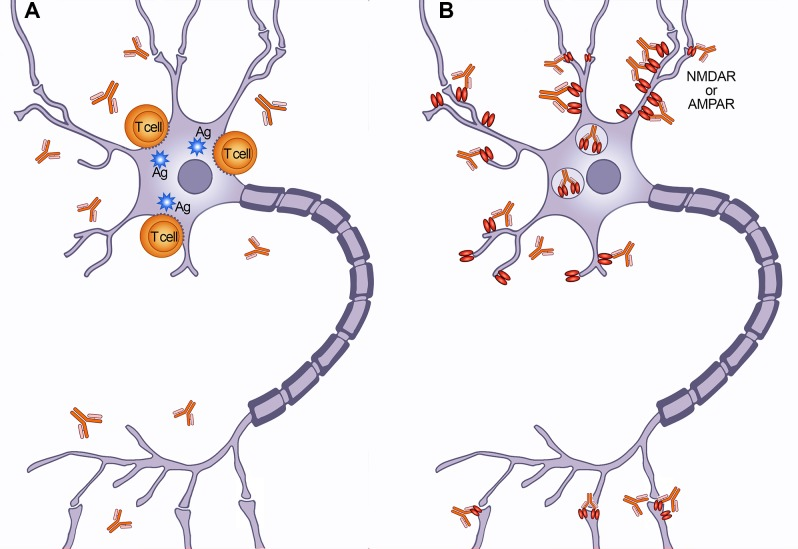
\includegraphics[width=0.85\textwidth]{abbildungen/AE2Bild.jpg} % Lädt das Bild, skaliert es auf 80% der Textbreite
	\caption{ A: onkoneurale AK richten sich gegen intrazelluläre Proteine. B: aAK gegen neuronale Oberflächenantigene. \parencite{PNSChannelBild2017}} % Die Bildunterschrift
	\label{fig:AE2} % Ein Label für Querverweise (z.B. "siehe Abbildung \ref{fig:beispielbild}")
\end{figure}

Generell verlaufen AE in der Regel zunächst subakut bis chronisch. Über
den Langzeitverlauf von AE wurden bisher nur wenige Daten erhoben. Je
nach Zeitpunkt der Diagnosestellung und des Therapiebeginns kommt es bei
nicht-paraneoplastischen AE allerdings meist zur vollständigen oder
teilweisen Erholung.\footcite[S.~533]{Heine2022}
Kurz nach der Akutphase sind die Genesungschancen für Patienten zwar am
höchsten, dennoch lassen sich noch nach mehreren Jahren Verbesserungen
der kognitiven Fähigkeiten
verzeichnen.\footcite[S.~534]{Heine2022}
Paraneoplastische Enzephalitiden hingegen sind meist Tumor-assoziiert,
sprechen daher selten auf immunwirksame Behandlungen an und erzeugen oft
schwere und bleibende neurologische
Ausfallerscheinungen.\footcite{UniHeidelbergAE2026}

Da sich diese Arbeit mit der Caspr2-AE auseinandersetzt, ist
im Folgenden zunächst von nicht-paraneoplastischen Enzephalitiden
die Rede.

Zur Diagnostik einer AE hilft die Zuordnung erhobener Befunde in Kategorien. Diese Befunde stammen unter anderem aus der
klinischen Analyse der Symptome und möglicher Syndrome,
Magnetresonanztomographie (MRT), Liquoranalyse,
Elektroenzephalogramm (EEG) und Antikörperdiagnostik. In Graus et al.\ (2016) findet sich ein klinischen Diagnosealgorithmus, der ausgehend vom Verdacht auf eine autoimmune Enzephalitis verschiedene klinisch charakterisierbare Syndrome, sowie antikörperassoziierte und antikörpernegative Erkrankungen berücksichtigt.
\footcite[S.~394]{Graus2016}

Wie in Abbildung \ref{fig:AE1} zu erkennen ist, sollte bei Verdacht einer AE eine Diagnostik 
auf zugrundeliegende aAK initiiert werden. Dies
sollte in Abhängigkeit von klinischen Syndromen und Zusatzbefunden (siehe oben) geschehen. Zwar
kann die Diagnose einer AE ohne Nachweis von AK bei AE-typischen
Veränderungen im Liquor, MRT und EEG sowie dem zusätzlichen Ausschluss
wichtiger Differentialdiagnosen gestellt werden, allerdings führt erst
der Nachweis von aAK zu einer sicheren
Diagnose.\footcites[S.~394]{Graus2016}{GenerateNet2026}

\begin{figure}[h] % [h] versucht, das Bild hier zu platzieren (hier), [t] für oben, [b] für unten
	\centering % Zentriert das Bild horizontal
	
\includegraphics[width=0.85\textwidth]{AE1bild.png} % Lädt das Bild, skaliert es auf 80% der Textbreite
	\caption{ Vereinfachter schematischer Ablauf der Diagnose und
		Differentialdiagnose autoimmuner
		Enzephalitiden. \parencite{GenerateNetBild2026}} % Die Bildunterschrift
	\label{fig:AE1} % Ein Label für Querverweise (z.B. "siehe Abbildung \ref{fig:beispielbild}")
\end{figure}

\clearpage
Die Therapie von AE sollte auch ohne bestätigten Antikörpernachweis
frühestmöglich beginnen, um die weitere Entzündung des Gehirns durch das
Immunsystem zu verhindern. Dabei ist die Therapie in zwei Bereiche mit
verschiedenen Therapiemöglichkeiten unterteilt. Die Erstlinientherapie,
bspw.\ mit hochdosierten Steroiden, dient zunächst der Abschwächung der
Immunreaktion. Um die Erkrankung langfristig unter Kontrolle zu bekommen, ist eine
weitere Therapie mit Medikamenten, die gezielt AK-produzierende B-Zellen beseitigen,
sinnvoll. Zusätzlich zu einer Immuntherapie erfolgt meist eine
symptomatische Behandlung. Im Falle von Tumoren müssen diese zunächst entfernt oder behandelt werden. 
Es werden ebenfalls nichtmedikamentöse
Maßnahmen, wie Physiotherapie oder neurologische Rehabilitation, zur
Förderung der funktionalen Fähigkeiten, die zuvor durch die AE gemindert wurden, im Alltag
angeraten.\footcite[S.~533]{Heine2022}
Einerseits, weil sich bei einzelnen AE auch nach mehreren Jahren
Verbesserungen von kognitiven Funktionen erkennen
lassen\footcite[S.~534]{Heine2022}, andererseits weil selbst nach einer
Verbesserung der Symptomatik ein Rückfall nicht auszuschließen
ist.\footcite[S.~11]{Lancaster2015}


AE werden nach den auslösenden aAK charakterisiert und benannt. Die
Caspr2-Enzephalitis wird durch die anti-Caspr2-aAK ausgelöst. Sie geht
häufig einher mit bestimmten Symptomen und Syndromen, die jedoch von
Patient zu Patient variieren.\footcite[S.~525--526]{VanSonderen2016}

Dazu zählen:
\begin{itemize}
	\item Übererregbarkeit des PNS:
	\begin{itemize}
		\item Neuromyotonie (Die Überaktivität der Nerven, welche die Muskelfasern anregen. Es entwickelt sich eine fortschreitende Versteifung der Muskeln, ein anhaltendes Muskelzittern sowie Zuckungen und Krämpfe.)\footcite{MSDNeuromyothonie2024}
		\item neuropathische Schmerzen, sowie Gelenk-, Muskel- und
		Brustschmerzen
	\end{itemize}
	\item limbische Enzephalitis
	\item Morvan-Syndrom (Kombination aus neuropsychiatrischen Symptomen
	[Schlafstörung, kognitive Defizite], autonomer
	Funktionsstörung [Störung von unwillkürlichen Körperprozessen, wie Herzschlag] und Neuromyotonie)
	\item Gewichtsverlust\footcites[S.~523; 526]{VanSonderen2016}%
	[S.~527; 530]{Heine2022}
\end{itemize}

Die meisten nicht-paraneoplastischen AE gehen deutlich seltener mit
Tumoren einher als paraneoplastische AE, so auch die
Caspr2-Enzephalitis. Ist dies dennoch der Fall, dann handelt es sich
meist um Tumore der Thymusdrüse.\footcite[S.~527; 530]{Heine2022}

Es lässt sich feststellen, dass überwiegend ältere Männer von der
Caspr2-Enzephalitis betroffen sind, wobei das durchschnittliche Alter zum
Zeitpunkt des Auftretens der Symptome 66~Jahre
betrug.\footcite[S.~522--523; 526]{VanSonderen2016}

\section{Wirkungsweise der Anti-Caspr2-Autoantikörper}

Die Anti-Caspr2-aAK binden an die
extrazellulären Domänen von Caspr2 auf der Oberfläche von Nervenzellen.
Sie binden insbesondere an die Discoidin- und
Laminin-1-Domänen.\footcite[S.~6]{Olsen2015}

AK werden im Allgemeinen je nach ihrer Effektorfunktion in vier
Immunglobulin-Subklassen (IgG1--4)
unterschieden.\footcite{Mitrevski}
Die AK der Klasse IgG4 lösen kaum Entzündungsreaktionen aus, sondern
blockieren die Funktionen der Zielstrukturen, sodass beispielsweise die
Bindung von Antigenen an andere Antigene verhindert
wird.\footcite{AntwerpesIgG4}
Die IgG1-AK sind mit verstärkten Entzündungsreaktionen und
Komplementaktivierung assoziiert.\footcite{Mitrevski}
Der Test auf IgG4 ist in der Studie von van~Sonderen et~al.\ (2016) in
100\,\% der Fälle, in denen die Caspr2-Enzephalitis auftrat, positiv
ausgefallen. 63\,\% der Testergebnisse lieferten ein positives Ergebnis
bei der IgG-Klasse IgG1. 19~Patientinnen und Patienten wurden bezüglich
der IgG-Klasse der AK getestet.\footcite[S.~524]{VanSonderen2016}

Die Rückfallquote scheint ebenfalls hoch zu sein. In der klinischen
Forschung von van~Sondern et~al.\ (2016) liegt sie bei 25\,\%, wobei die
Rückfälle bis zu sieben Jahren nach Auftreten der Erkrankung eingetreten
sind.\footcite[S.~524]{VanSonderen2016}
Dabei sind die Anti-Caspr2-aAK nicht für eine geminderte Expression von
Caspr2 an der Zelloberfläche verantwortlich. Caspr2 wird durch die aAK
funktionell blockiert, sodass es nicht mehr mit Contactin2 interagieren
kann.\footcite[S.~6--7]{Patterson2018}\\
\\
Die Kaliumkanäle (Kv1.1/1.2), die normalerweise durch den Komplex in den
juxtaparanodalen Regionen der Axone verankert sind, verlieren ihre
räumliche Organisation.\footcites{Mitrevski}[S.~8]{Patterson2018}\\
\\
Wie in Kapitel~2.1.2 beschrieben, sind Kaliumkanäle für die
Repolarisation nach einem Aktionspotential essenziell. Bei gestörter
Verankerung kommt es zu axonaler Hyperexzitabilität, die Neuronen werden
also zu lange
erregt.\footcite[S.~525--526]{VanSonderen2016}
Dies erklärt die Symptome Neuromyotonie, Übererregbarkeit und
neuropathische Schmerzen aus Kapitel~4.1. Während die axonale Pathophysiologie gut verstanden ist,
ist die Wirkung von Anti-Caspr2-aAK an den Synapsen noch wenig
charakterisiert.
